\documentclass[a4paper,oneside,titlepage,11pt]{article}
\usepackage{xltxtra}
\usepackage{xgreek}
\setmainfont[Mapping=tex-text]{Meslo LG M} %Courier New for programing
\usepackage{amsfonts}
\usepackage{listings}
\usepackage{color}

\usepackage{graphicx}
\usepackage{pdflscape}

\usepackage{enumerate}

\usepackage{svg}

\usepackage{geometry}
\geometry{a4paper, portrait, margin=1in}

\definecolor{codegreen}{rgb}{0,0.6,0}
\definecolor{codegray}{rgb}{0.5,0.5,0.5}
\definecolor{codepurple}{rgb}{0.58,0,0.82}
\definecolor{backcolour}{rgb}{0.95,0.95,0.95}
\definecolor{com}{rgb}{0.55,0.55,0.55}

\title{Πρώτο σετ ασκήσεων}
\date{}
\author{}
 
\lstdefinestyle{mystyle}{
    %backgroundcolor=\color{backcolour},   
    commentstyle=\color{codegreen},
    keywordstyle=\color{magenta},
    numberstyle=\tiny\color{codegray},
    stringstyle=\color{codepurple},
    basicstyle=\footnotesize,
    breakatwhitespace=false,         
    breaklines=true,                 
    captionpos=b,                    
    keepspaces=true,                 
    numbers=left,                    
    numbersep=5pt,                  
    showspaces=false,                
    showstringspaces=false,
    showtabs=false,                  
    tabsize=2
}

\lstdefinestyle{mystyle2}{
	numberstyle =\tiny\color{codegray},
    basicstyle=\small,
    breakatwhitespace=false,         
    breaklines=true,                 
    captionpos=b,                    
    keepspaces=true,                 
    numbers=left,                    
    numbersep=5pt,                  
    showspaces=false,                
    showstringspaces=false,
    showtabs=false,                  
    tabsize=2
}
 
 \lstdefinestyle{mystyle3}{
	numberstyle =\tiny\color{codegray},
    basicstyle=\footnotesize,
    commentstyle=\color{codegreen},
    breakatwhitespace=false,         
    breaklines=true,                 
    captionpos=b,                    
    keepspaces=true,                 
    numbers=left,                    
    numbersep=5pt,                  
    showspaces=false,                
    showstringspaces=false,
    showtabs=false,                  
    tabsize=2
}

\lstdefinestyle{style}{
    backgroundcolor=\color{backcolour},   
    commentstyle=\color{codegreen},
    keywordstyle=\color{magenta},
    numberstyle=\tiny\color{codegray},
    stringstyle=\color{codepurple},
    basicstyle=\footnotesize,
    breakatwhitespace=false,         
    breaklines=true,                 
    captionpos=b,                    
    keepspaces=true,                 
    numbers=left,                    
    numbersep=5pt,                  
    showspaces=false,                
    showstringspaces=false,
    showtabs=false,                  
    tabsize=2
}

 \lstset{style=style}

%\pagestyle{headings} 

\usepackage{graphicx}
\graphicspath{ {images/} }
 
\begin{document}

\begin{center}
{\small ΠΑΝΕΠΙΣΤΗΜΙΟ ΠΑΤΡΩΝ - ΠΟΛΥΤΕΧΝΙΚΗ ΣΧΟΛΗ\\
ΤΜΗΜΑ ΜΗΧΑΝΙΚΩΝ Η/Υ ΚΑΙ ΠΛΗΡΟΦΟΡΙΚΗΣ} \\
\vspace{0.3cm}
\textbf{ΕΡΓΑΣΤΗΡΙΟ ΒΑΣΕΩΝ ΔΕΔΟΜΕΝΩΝ}
\\
\textbf{PROJECT 2016-2017}
\\ \leavevmode \\
\end{center}

\begin{flushright}
\textbf{Εργασία Φοιτητών:}\\
Σταυρούλα Δρίτσα, ΑΜ. 6040\\
\texttt{dritsa@ceid.upatras.gr}

Δαμιανός Ντούμη Σιγάλας, ΑΜ. 6157\\
\texttt{nsigalas@ceid.upatras.gr}
\end{flushright}



\noindent\textbf{Ερώτημα 1} 

Το ER και το σχεσιακό διάγραμμα παρατίθενται στο τέλος της παρούσας αναφοράς μαζί με τις παραδοχές για το ER. Αρχεία υψηλότερης ανάλυσης βρίσκονται στο φάκελο με όνομα ``ΔΙΑΓΡΑΜΜΑΤΑ''.
\vspace{0.6cm}

\noindent\textbf{Ερώτημα 2} 

Αρχικά για να συνδεθούμε με την mysql που τρέχει σε τοπικό server με λειτουργικό σύστημα Windows, χρησιμοποιούμε την εξής σύνταξη:
\begin{center}
\texttt{mysql -u \textit{username} -p --default-character-set=utf8}
\end{center}

Στο αρχείο \texttt{create.sql} υπάρχουν οι κατάλληλες SQL εντολές για την δημιουργία των πινάκων που υλοποιούν το σχήμα της βάσης δεδομένων μας. Αντίστοιχα στο \texttt{insert.sql} αρχικοποιούμε τους πίνακες της βάσης με τα κατάλληλα δεδομένα που μας επιτρέπουν τον έλεγχο της σωστής λειτουργίας της και την εκτέλεση των ερωτημάτων.

Τα δεδομένα που χρησιμοποιούμε προέρχονται στο μεγαλύτερο μέρος τους από τον ιστότοπο της Superleague και αφορούν το πρωτάθλημα του έτους 2016-17. Όπου χρειαστεί έχουμε προσθέσει ή τροποποιήσει στοιχεία ώστε να μας διευκολύνουν στις δοκιμές μας.
\vspace{0.6cm}

\noindent\textbf{Ερώτημα 3} 
\vspace{0.3cm}

\noindent 1. Ποιά είναι τα βιογραφικά του προέδρου και του προπονητή της ομάδας με τις περισσότερες νίκες στο πρωτάθλημα;
\lstinputlisting[language=SQL]{sql/query1.sql}
\vspace{0.3cm}

Σύμφωνα με την περιγραφή των προδιαγραφών του project ο πρόεδρος δεν διαθέτει βιογραφικό επομένως για λόγους ευκολίας επιλέγεται να εμφανίζεται το όνομα του.
\vspace{0.3cm}

\pagebreak
\noindent 2. Ποιός παίκτης σημείωσε τα περισσότερα τέρματα στο πρωτάθλημα και πόση είναι η διαφορά τερμάτων από το δεύτερο παίκτη σε τέρματα;
\lstinputlisting[language=SQL]{sql/query2.sql}

\noindent 3. Σε κάθε ομάδα ποιοί παίκτες είναι οι τρεις με τα περισσότερα τέρματα και ποιοί είναι οι φίλαθλοι (ονοματεπώνυμα) που τους έχουν επιλέξει ως αγαπημένους;
\lstinputlisting[language=SQL]{sql/query3.sql}
\vspace{0.3cm}

\noindent 4. Για κάθε ομάδα πόσα είναι τα εισιτήρια διαρκείας και ποιοι οι φίλαθλοι που τα έχουν αγοράσει;
\lstinputlisting[language=SQL]{sql/query4.sql}
\vspace{0.3cm}

\pagebreak
\noindent 5. Ποιός είναι ο φίλαθλος που χρησιμοποιήσε τις περισσότερες φορές το εισιτήριο διαρκείας, αν έχει λάβει μήνυμα ανανέωσης του εισιτηρίου του, σε ποιούς αγώνες δεν πήγε και ποιές ήταν οι ημερομηνίες των αγώνων αυτών;
\lstinputlisting[language=SQL]{sql/query5.sql}
\vspace{0.3cm}

\pagebreak
\noindent 6. Ποιά είναι η έδρα, ο πρόεδρος, και ο προπονητής της ομάδας που έχει την μέγιστη διαφορά μεταξύ των τερμάτων που έχει δεχθεί μείον των τερμάτων που έχει σημειώσει;
\lstinputlisting[language=SQL]{sql/query6.sql}
\vspace{0.3cm}

\noindent 7. Δίνοντας ως όρισμα σε μια stored procedure το όνομα μιας ομάδας να επιστρέφονται οι 3 αγώνες με τις περισσότερες πωλήσεις απλών εισητηρίων στους φιλάθλους της είτε ήταν εντός είτε εκτός έδρας.
\lstinputlisting[language=SQL]{sql/query7.sql}
\vspace{0.3cm}

\noindent 8. Trigger που να αποτρέπει την εισαγωγή πενταμελούς διαιτησίας, στην οποία ενας διαιτητής αναλαμβάνει παραπάνω από έναν ρόλο.  
\lstinputlisting[language=SQL]{sql/query8.sql}
\vspace{0.3cm}

\noindent 9. Stored Procedure που εμφανίζει τα έσοδα από τα εισιτήρια (απλα και διαρκείας) μιας ομάδας που δίνεται ως όρισμα.
\lstinputlisting[language=SQL]{sql/query9.sql}
\vspace{0.3cm}

\noindent 10. Ερώτημα που εμφανίζει τις διακριτές πεντάδες διαιτητών που έχουν συμμετάσχει στην διαιτησία κάποιου αγώνα.
\lstinputlisting[language=SQL]{sql/query10.sql}
\vspace{0.3cm}

\newpage

\noindent\textbf{Ερώτημα 4} 
\vspace{0.3cm}

\noindent Για την ανάπτυξη του γραφικού περιβάλλοντος της εφαρμογής μας επιλέξαμε τη χρήση της βιβλιοθήκης γραφικών JavaFX Release 8, που είναι διαθέσιμη μαζί με τις εκδόσεις του JRE 8 και JDK 8 της Java. Συγκεκριμένα η ανάπτυξη της εργασίας έγινε χρησιμοποιώντας το IDE IntelliJ IDEA 2017.1.4 μαζί με το jdk 1.8.0\_111.

\vspace{0.3cm}
\noindent\textbf{Έναρξη του προγράμματος} 
\vspace{0.3cm}

\noindent Με την έναρξη της εκτέλεσης του προγράμματος εμφανίζεται το εξής παράθυρο:

\begin{center}
 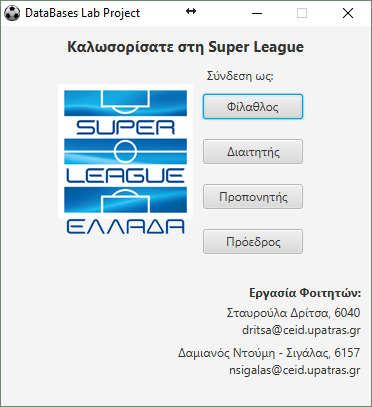
\includegraphics[scale=1]{screens/1_start.PNG} 
\end{center} 

\noindent Απο αυτό ο χρήστης καλείται να επιλέξει τον ρολο με τον οποίο επιθυμεί να συνδεθεί στη βάση δεδομένων ώστε να του εμφανιστεί η κατάλληλη διεπαφή. Στη συνέχεια θα εξετάσουμε τα διαφορετικά είδη διεπαφών:

\vspace{0.3cm}

\noindent\textbf{i. Φίλαθλος} 
\vspace{0.3cm}

\noindent Στο επάνω μέρος του παραθύρου ζητάμε από τον χρήστη να πληκτρολογήσει το id του φιλάθλου για τον οποίο επιθυμεί να ανακτήσει τις πληροφορίες από την βάση δεδομένων. Παράλληλα πρέπει να εισάγει και μια ημερομηνία η οποία θα χρησιμοποιηθεί ως σημείο αναφοράς για τον υπολογισμό παρελθοντικών και μελλοντικών δεδομένων. 
\vspace{0.3cm}

\noindent Ακριβώς απο κάτω εμφανίζονται τα στοιχεία του φιλάθλου για το δοθέν id όπως το όνομα, η ομάδα που υποστηρίζει, η διαφορά τερμάτων της και αν είναι κάτοχος κάρτας διαρκείας. Σε περίπτωση που κατέχει διαρκείας εμφανίζεται επιπλέον ένδειξη με τις διαθέσιμες θέσεις στον αμμέσως επόμενο προγραμματισμένο αγώνα ο οποίος πραγματοποιείται εκτός έδρας της ομάδας του. Επίσης η εισαγωγή λανθασμένου id θα οδηγήσει στην εμφάνιση κατάλληλου μηνύματος.

\begin{center}
 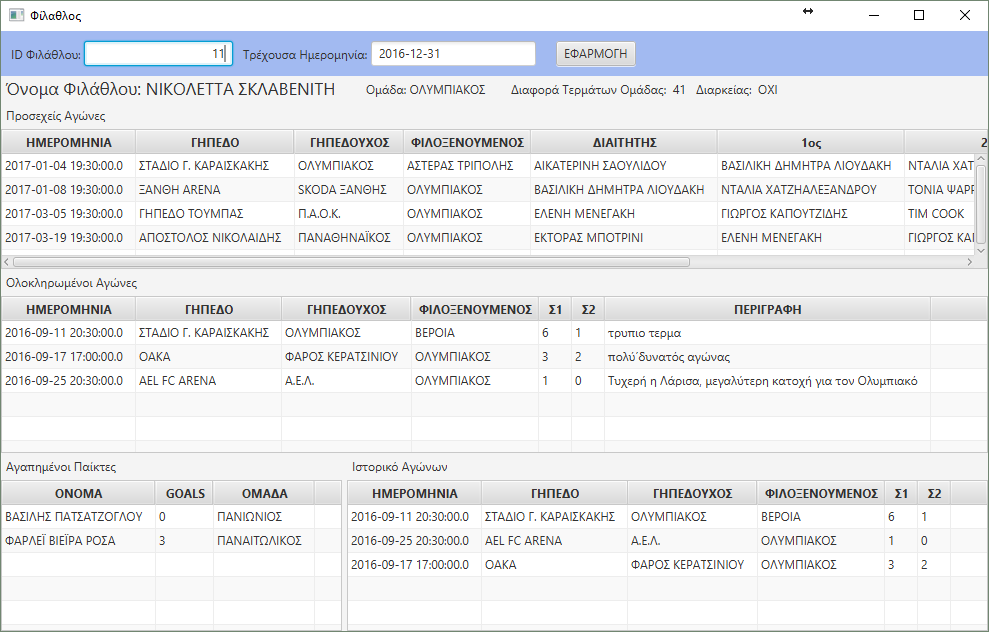
\includegraphics[scale=0.6]{screens/2_fan.PNG} 
\end{center} 

\noindent Στη συνέχεια εμφανίζονται με την μορφή πινάκων στοιχεία για τους προσεχείς και ολοκληρωμένους αγώνες, τους αγαπημένους παίκτες του φιλάθλου (οι οποίο δεν ανήκουν απαραιτήτως στην ίδια ομάδα)καθώς και το ιστορικό των αγώνων που έχει παρακολουθήσει. 

\vspace{0.3cm}

\noindent\textbf{ii. Διαιτητής} 

\begin{center}
 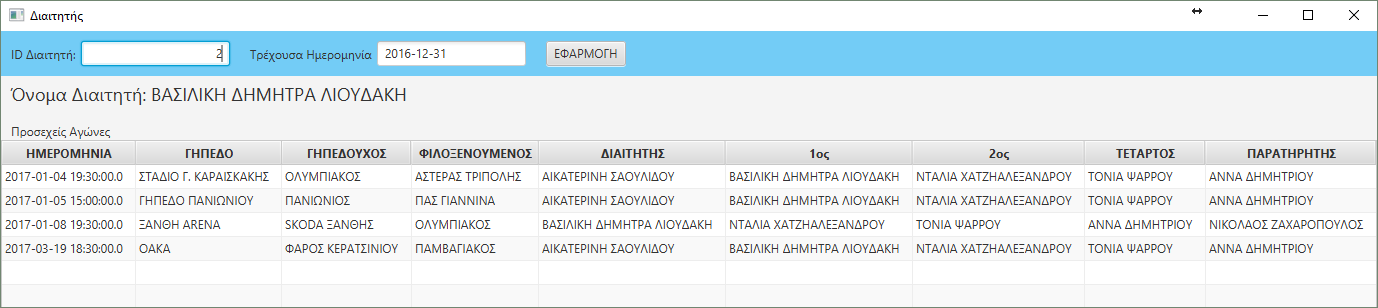
\includegraphics[scale=0.45]{screens/3_referee.PNG} 
\end{center} 

\noindent Παρομοίως με τον φίλαθλο, στη διεπαφή που αφορά τους διαιτητές ζητείται το προς αναζήτηση id και η τρέχουσα ημερομηνία. Εφόσον τα δεδομένα που θα δοθούν είναι έγκυρα, εμφανίζονται οι μελλοντικοί αγώνες στους οποίους ο διαιτητής έχει οριστεί να συμμετέχει καθώς και η θέση του στην πεντάδα της διαιτησίας.

\newpage

\noindent\textbf{iii. Προπονητής} 
\vspace{0.3cm}

\noindent Ο προπονητής βλέπει στοιχεία που αφορούν τους μελλοντικούς αγώνες και τους διαθέσιμους παίκτες. Οι αγώνες που έχουν πραγματοποιηθεί σε παρελθοντικό χρόνο, χωρίζονται στις νίκες, στις ήττες και στις ισοπαλίες. Ακόμα εμφανίζονται οι παίκτες που έχει στη διάθεσή του, ενώ έχει την δυνατότητα να προσθέσει νέους παίκτες στην ομάδα του.

\begin{center}
 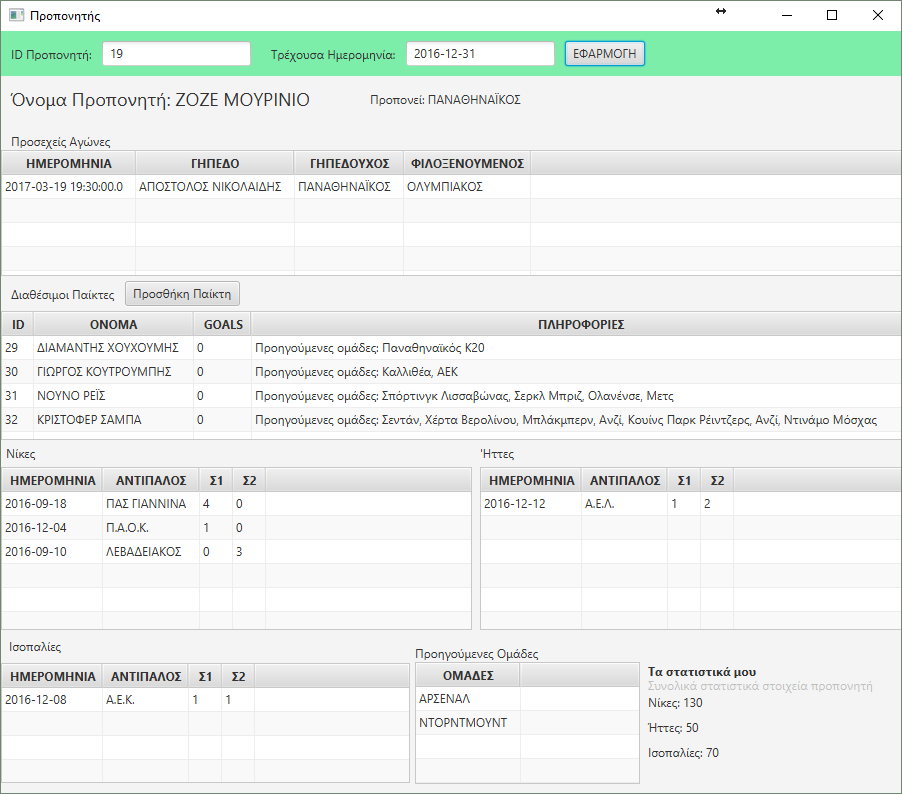
\includegraphics[scale=0.65]{screens/4_coach.PNG} 
\end{center} 

\noindent Επίσης, εμφανίζονται στοιχεία που συνθέτουν το προφίλ του όπως οι ομάδες που έχει εργαστεί ως προπονητής στο παρελθόν και τα συνολικά στατιστικά του.
\vspace{0.3cm}

\noindent Πατώντας το κουμπί ``Προσθήκη Παίκτη'' εμφανίζεται ενα αναδυώμενο παράθυρο στο οποίο ο χρήστης (προπονητής) καλείται να συμπληρώσει τα στοιχεία του νέου παίκτη.

\begin{center}
 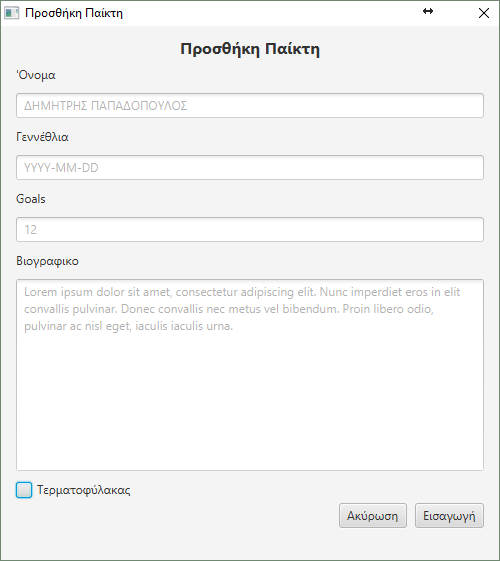
\includegraphics[scale=0.76]{screens/4_create.PNG}  
\end{center} 

\noindent Σε περίπτωση εισαγωγής μη έγκυρων δεδομένων που οδηγούν σε αποτυχία εισαγωγής της νέας εγγραφής, υπάρχει η κατάλληλη ενημέρωση του χρήστη:

\begin{center} 
 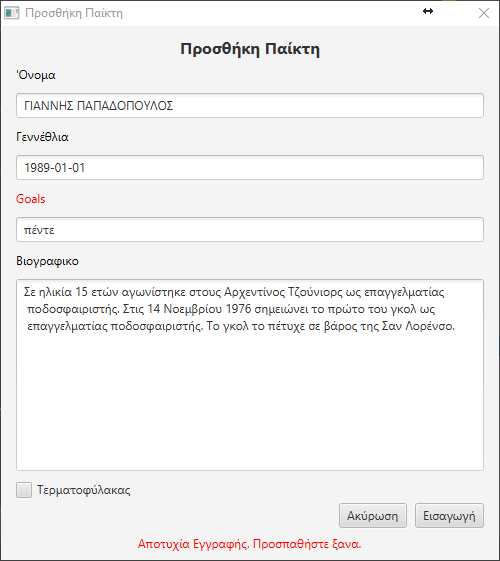
\includegraphics[scale=0.76]{screens/4_create_error.PNG} 
\end{center} 


\noindent\textbf{iv. Πρόεδρος} 
\vspace{0.3cm}

\noindent Για τον πρόεδρο, οποίος χαρακηρίζεται μοναδικά από το όνομα του και το όνομα της ομάδας στην οποία είναι πρόεδρος, εμφανίζονται στοιχεία σχετικά με τις πωλήσεις όλων των τύπων εισητηρίων. Ταυτόχρονα πατώντας το κουμπί ``Στείλε Προσφορές'', εμφανίζονται τα ονόματα των φιλάθλων οι οποίοι δικαιούνται προσφορά. 

\begin{center}
 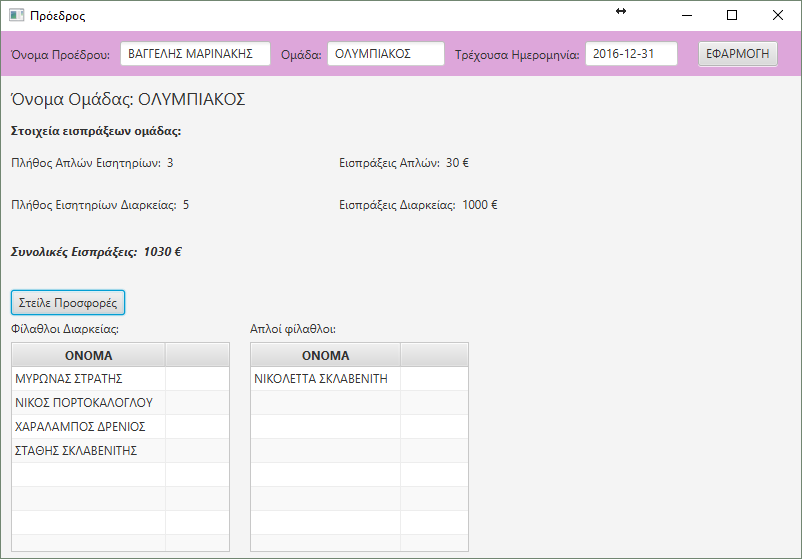
\includegraphics[scale=0.75]{screens/5_owner.PNG} 
\end{center} 



%\leavevmode \newline


\newpage


{\Large \noindent \textbf{Παραδοχές στο ER}}

\vspace{0.3cm}

\noindent Αρχικά για να αναπαραστήσουμε ολική συμμετοχή σε μία σχέση, χρησιμοποιείται ευθεία bold γραμμή (αντί διπλής).

\begin{enumerate}
\item Μία ομάδα δεν μπορεί να μην έχει έδρα.
\item Το όνομα ενός γηπέδου είναι μοναδικό.
\item Δεν υπάρχει εισιτήριο διαρκείας που να μην ανήκει σε κάποιον φίλαθλο.
\item Δεν υπάρχει ομάδα χωρίς πρόεδρο.
\item Επιτρέπεται η ύπαρξη προπονητή που δεν προπονεί ομάδα.
\item Θεωρούμε ότι ένας διαιτητής συμμετέχει σε ένα πενταμελές σχήμα διαιτησίας, το οποίο σφυρίζει έναν αγώνα. 
\item  Για κάθε σχήμα διαιτησίας πρωτεύον κλειδί είναι το σύνολο των γνωρισμάτων του, καθώς κάθε πεντάδα διαιτητών είναι μοναδική και μπορεί να συμμετέχει σε πάνω από έναν αγώνες.
\item  Όπου υπάρχει ως γνώρισμα η ηλικία, αυτή αναπαρίσταται ως παραγόμενο γνώρισμα της ημερομηνίας γέννησης.
\item  Όποια οντότητα δεν είχε προφανές πρωτεύον κλειδί προσθέσαμε ένα μοναδικό ID.

\end{enumerate}

\begin{landscape}
\begin{figure}
\centering
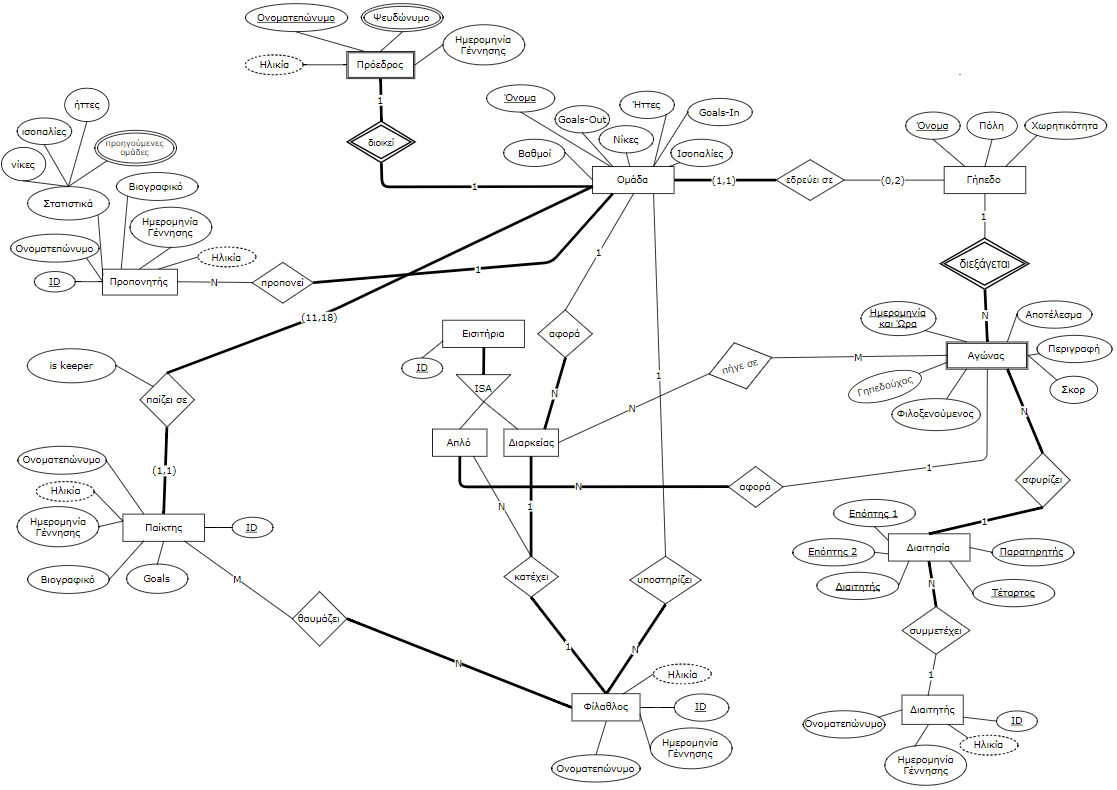
\includegraphics[scale=0.75]{er.png} 
\caption{Διάγραμμα ER}
\end{figure}
\end{landscape}

\begin{landscape}
\begin{figure}
\centering
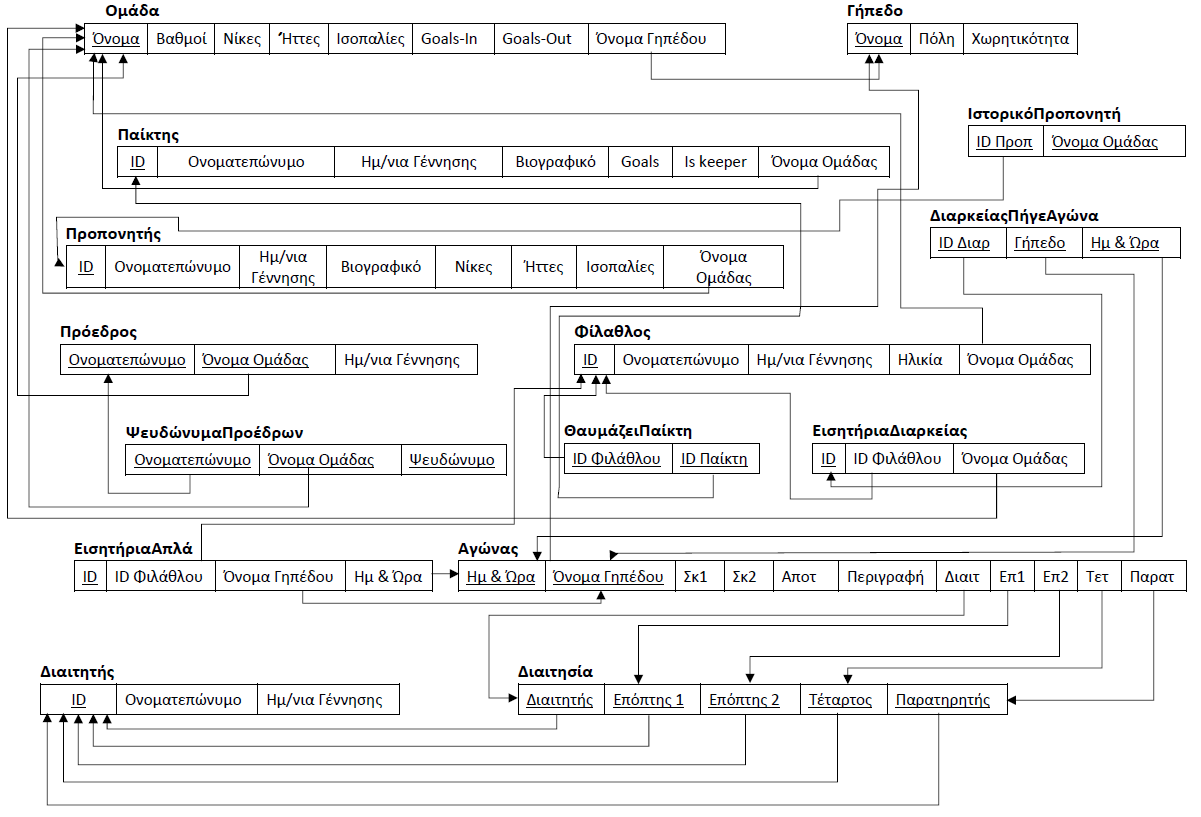
\includegraphics[scale=0.75]{sxesiako} 
\caption{Σχεσιακό Διάγραμμα}
\end{figure}
\end{landscape}

\end{document}